% =====================================================================
% SpinVL -- CVPR submission draft (SELF-CONTAINED / FALLBACK BUILD)
%
% This file compiles with a plain TeX Live / MiKTeX installation and
% reproduces the CVPR two-column layout (10pt Times, 6.875 x 8.875 in
% text block) without requiring the official kit.
%
% >>> For the OFFICIAL submission build, use main_cvpr_official.tex
%     together with cvpr.sty from the CVPR author kit instead.
% =====================================================================
\documentclass[10pt,twocolumn,letterpaper]{article}

\usepackage[letterpaper,text={6.875in,8.875in},centering,top=1in]{geometry}
\usepackage{times}
\usepackage{graphicx}
\usepackage{amsmath,amssymb}
\usepackage{booktabs}
\usepackage{multirow}
\usepackage{array}
\usepackage{xcolor}
\usepackage[font=small,labelfont=bf,textfont=small]{caption}
\usepackage[numbers,sort&compress]{natbib}
\usepackage[hidelinks]{hyperref}

\graphicspath{{figures/}}
\setlength{\columnsep}{0.31in}
\renewcommand{\arraystretch}{1.05}

\newcommand{\modelname}{SpinVL}
\newcommand{\ie}{\emph{i.e.}}
\newcommand{\eg}{\emph{e.g.}}

\begin{document}

% ---------------------------------------------------------------------
% Title block (full width)
% ---------------------------------------------------------------------
\twocolumn[{
\begin{center}
{\LARGE\bfseries \modelname: Turning Frozen Text LLMs into Vision-Language\\[2pt]
Models with Zero Visual Tokens in the Backbone\par}
\vspace{10pt}
{\large Anonymous CVPR submission\par}
\vspace{4pt}
{\small Paper ID 0000\par}
\end{center}
\vspace{6pt}
\begin{center}
\begin{minipage}{0.90\textwidth}
\small
\textbf{Abstract}
\vspace{3pt}

Vision-language models (VLMs) built by concatenating visual tokens into a
frozen or fine-tuned LLM pay a steep price: attention cost grows with image
resolution, and adapting the backbone erodes the language model's original
text reasoning. Parameter-rotation methods remove visual tokens from the
backbone, but still depend on a heavy external vision tower, and they
deteriorate once the model generates autoregressively on its own. We introduce
\modelname, a framework that converts a completely frozen pure-text LLM into a
VLM that keeps \textbf{zero visual tokens in the backbone} and, in its
strongest configuration, \textbf{removes the external vision tower entirely}.
\modelname{} rests on two mechanisms. A \emph{dual-tier orthogonal rotation}
architecture first repurposes the student's own first $K{=}4$ layers as a
built-in vision encoder through static Cayley rotation and channel-wise
scaling ($2.4$M parameters), then discards every image token and modulates the
deeper frozen layers with dynamic block-diagonal rotations generated by
multi-frequency or spatial-anchor queries. Because the text pathway is left
untouched, pure-text behaviour is bit-exact, whereas merging the same vision
adapters into the backbone collapses GSM8K from $70.4\%$ to $0.0\%$.
Second, \emph{online policy distillation} (VL-OPD) supervises the student's
own rollouts with token-level KL from a stronger VLM, which lifts free-form
generation by up to $+9.9$ points. With the same training data, steps, and
frozen base model, \modelname{} outperforms a token-concatenation LLaVA
baseline on visual perception and anti-hallucination
($44.37\%$ vs.\ $41.35\%$), matches it on the average of perception,
hallucination and mathematical reasoning ($35.90\%$ vs.\ $35.87\%$), is
strictly better than single-frequency rotation and LoRA-based built-in
encoders, and does so with $74.2\%$ fewer FLOPs and $100\%$ preserved text
ability.
\end{minipage}
\end{center}

\vspace{10pt}
}]

\section{Introduction}
\label{sec:intro}

\begin{figure*}[t]
\centering
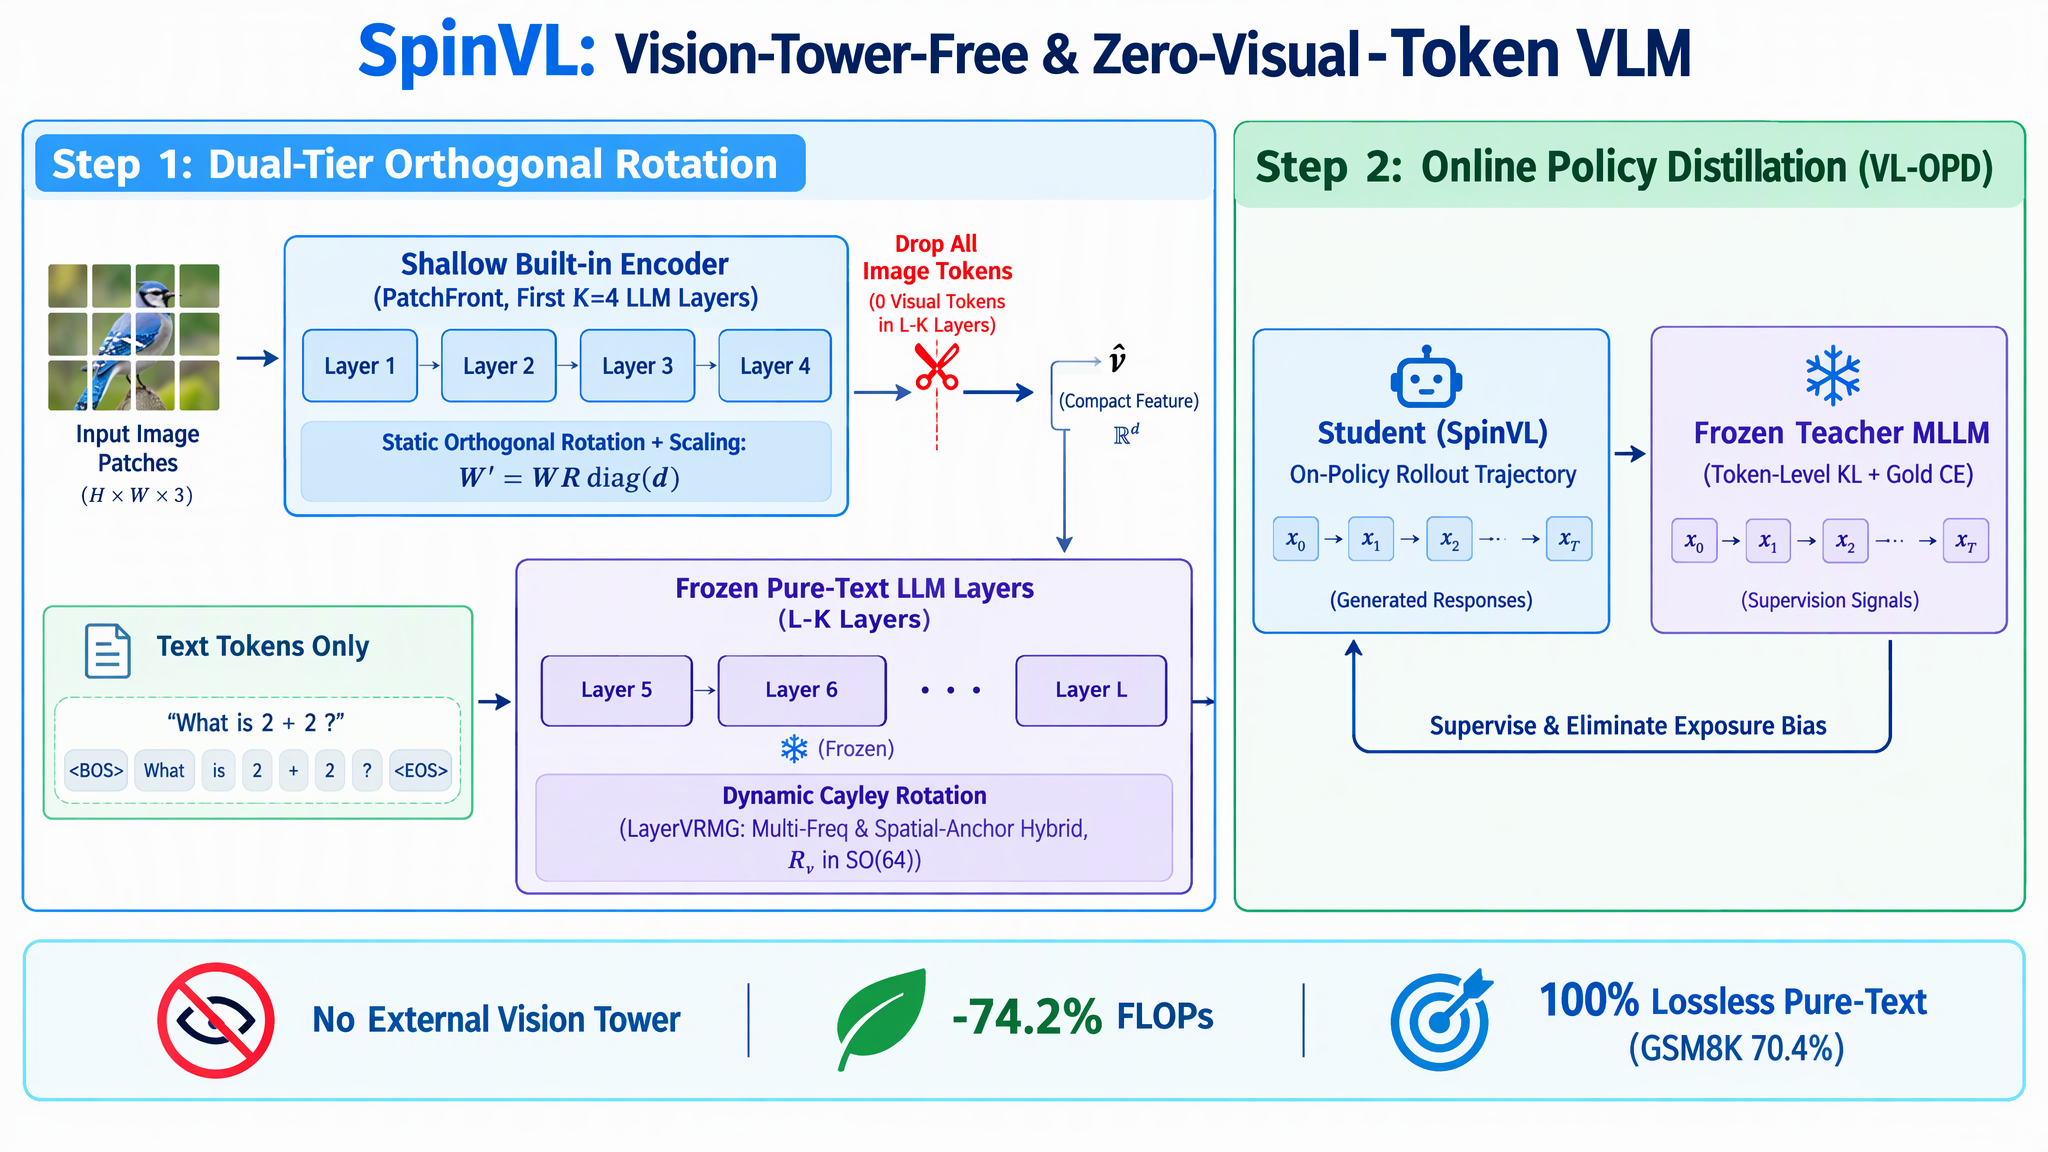
\includegraphics[width=0.98\textwidth]{fig_architecture.png}
\caption{\textbf{Overview of \modelname.} A completely frozen pure-text LLM is
turned into a VLM without any visual token inside the deeper backbone.
\emph{Step~1 (dual-tier orthogonal rotation):} the student's own first
$K{=}4$ layers act as a built-in vision encoder with static Cayley rotation
and channel scaling; all image tokens are discarded after layer $K$, and a
compact cell feature drives dynamic block-diagonal rotations in the remaining
layers. \emph{Step~2 (online policy distillation):} the student samples its
own trajectories and is supervised token-by-token by a stronger VLM, which
removes the exposure bias of teacher-forced training. The text pathway is
never modified, so pure-text behaviour is bit-exact.}
\label{fig:arch}
\end{figure*}

Feeding images to a language model is usually done by concatenation: a vision
encoder, often a full ViT with hundreds of millions of parameters, turns the
image into a sequence of tokens that is prepended to the text and propagated
through every layer of the LLM~\citep{liu2023llava,liu2024improved}. This
recipe is simple and effective, but it couples image resolution to the cost of
the language model. At $4096$ patches, a $1.7$B student with $28$ layers
spends $9.85$ TFLOPs per forward pass, an order of magnitude more than the
text-only model would; the KV cache grows with the same factor. The usual
remedy, fine-tuning the backbone on image-text pairs, trades away a property
that is expensive to recover: the instruction-following and mathematical
ability of the original model.

An appealing alternative is to modulate weights instead of extending the
context. Rotation-based injection~\citep{rose2025} keeps the backbone free of
visual tokens by mapping visual features to block-diagonal orthogonal matrices
that rotate the inputs of linear projections. It inherits the text model
untouched and removes the quadratic cost of long visual sequences. Three
problems remain. First, the method still requires an external vision tower,
which is exactly the component one would like to delete when deploying a
single frozen LLM. Second, images are pooled into one static rotation, so
spatial detail is lost and the model cannot revisit a region. Third, the
model is trained with teacher forcing on ground-truth answers; at inference
time it must consume its own prefixes, and small early errors compound---we
observe degenerate repetitions and missing end-of-sequence tokens.

A parallel line of work replaces the vision tower with the LLM's own early
layers~\citep{vora2025}. This removes the tower but keeps the visual tokens
alive: they travel through all remaining layers, so no compute is saved, and
merging the resulting low-rank adapters into the backbone destroys text
reasoning (GSM8K drops from $70.4\%$ to $0.0\%$ in our controlled experiment).

This paper asks whether one can have all three properties at once: no
external vision tower, no visual token in the deeper backbone, and intact text
ability. \modelname{} answers affirmatively with a two-step framework
(Fig.~\ref{fig:arch}).

\textbf{Step~1: dual-tier orthogonal rotation.} We distinguish two tiers of
adaptation. In the shallow tier, the student's first $K$ layers are
repurposed as a vision encoder using \emph{static} orthogonal rotation
combined with a channel-wise diagonal scaling, which preserves angular
geometry yet, unlike a pure rotation, can rescale singular values. Only
$2.4$M parameters are involved. After layer $K$ every image token is dropped
and a compact set of cell features remains. In the deep tier, those features
generate \emph{dynamic} block-diagonal rotations for the remaining frozen
layers. We propose two complementary generators: a multi-frequency variant
that splits rotation blocks into low-, mid-, and high-frequency bands with
RoPE-style positional encodings, and a hybrid variant that adds a lightweight
cross-attention over a handful of spatial anchors. The two target different
abilities---multi-step diagram reasoning versus fine-grained perception---and
we report both.

Because rotations are applied through a context-local wrapper, the text
pathway is untouched: with the vision branch switched off the model is
bit-identical to the original LLM ($70.4\%$ GSM8K, $71.4\%$ ARC-C). This is
not true for additive adapters or for permanently merged rotations, whose text
accuracy collapses.

\textbf{Step~2: online policy distillation.} Offline teacher forcing trains
the model only on ground-truth prefixes. We therefore let the student roll out
its own answers and ask a stronger VLM to score exactly those tokens with a
full-vocabulary forward KL, anchored by a gold cross-entropy term. Five
hundred steps suffice to raise free-form generation by $+4.1$ to $+9.9$
points across benchmarks and to bring end-of-sequence termination above
$95\%$.

\textbf{Controlled evidence.} All models in our main table share the same
frozen base model, the same training mixture, and the same optimisation
budget; the token-concatenation baseline is retrained by us rather than quoted.
Under this protocol \modelname{} improves the average of perception and
anti-hallucination from $41.35\%$ to $44.37\%$ without any visual token in the
backbone, reaches $35.90\%$ on the average of perception, hallucination and
mathematical reasoning against $35.87\%$ for the token-concatenation
baseline, and, in the tower-free configuration, retains $97.4\%$ of that
baseline's score while using $74.2\%$ fewer FLOPs and running $19.5\%$ faster
at high resolution.

Finally, we characterise the limits of the paradigm instead of hiding them.
By re-training the concatenation baseline on identical data that includes
open-ended chart and document questions, we show that its accuracy on
character-level chart reading and OCR stays flat ($10.32\%$ and $1.10\%$),
while our model stays in the low single digits; adding the same data doubles
our geometry accuracy. Operator-level modulation therefore buys semantic
perception, hallucination resistance and diagram reasoning, but not dense
transcription, which appears to require per-position key-value addressing.

Our contributions are:
\begin{itemize}
\item A dual-tier orthogonal rotation architecture that keeps zero visual
tokens in the backbone and needs no external vision tower, using $2.4$M
static parameters to turn the student's first layers into a vision encoder and
discarding all image tokens thereafter.
\item Multi-frequency and spatial-anchor rotation generators for the deep
tier, together with a modality-decoupled wrapper that makes pure-text
behaviour bit-exact.
\item An online policy distillation stage that repairs autoregressive drift of
rotation-injected models with $500$ steps of on-policy token-level KL.
\item A controlled study against token concatenation, single-frequency
rotation and LoRA-based built-in encoders, covering $0.6$B--$8$B students,
three seeds, compute, latency, text retention, and an explicit statement of
the paradigm's operating envelope.
\end{itemize}

\section{Related Work}
\label{sec:related}

\paragraph{Token-concatenation VLMs.}
LLaVA-style models connect a pretrained vision encoder to an LLM through a
light projector and train on instruction data~\citep{liu2023llava,
liu2024improved}. Scaling this recipe mostly means scaling the visual token
count, which is precisely what makes inference expensive at high resolution.
Token-pruning and spatial-pooling methods such as FastV~\citep{chen2024fastv}
and locality-aware projectors~\citep{cha2024honeybee} compress the visual sequence
to a smaller token budget, but still keep visual tokens inside every backbone layer.
Our baselines cover both full-token concatenation and $32$-token pruning/pooling
under our exact data and compute budget so that comparisons are apples-to-apples.

\paragraph{Parameter-efficient and encoder-free adaptation.}
Encoder-free VLMs internalise visual processing into the LLM by duplicating
modality-specific weights~\citep{diao2024eve} or inserting low-rank
adapters~\citep{hu2021lora,vora2025} into the early layers and distilling a
vision tower. While this removes the external ViT, unfreezing copied layers
requires ratusan of millions of parameters, and permanently merging additive
adapters into a text model destroys arithmetic reasoning, which motivates a
multiplicative, context-gated form of adaptation.

\paragraph{Rotation-based injection.}
ROSE~\citep{rose2025} converts visual features into block-diagonal orthogonal
matrices and rotates linear inputs, so the backbone never sees a visual token.
The construction guarantees that activations preserve their norm, and it is
attractive because the text model remains intact. Its limitations---a static,
globally pooled rotation, dependence on an external tower, and exposure bias
under greedy decoding---are the starting point of this work. We keep the
orthogonal construction, make it dynamic and spatially addressable, remove the
tower, and add on-policy distillation.

\paragraph{Distillation for VLMs.}
Knowledge distillation transfers a teacher's output distribution or feature
geometry to a student~\citep{hinton2015distilling,park2019rkd}; sequence-level
and on-policy variants~\citep{kim2016sequence,gu2024minillm,agarwal2024gkd}
train on student-generated trajectories. Off-policy distillation on
ground-truth prefixes does not cover the states a model visits when it decodes
on its own, whereas mode-seeking reverse KL~\citep{gu2024minillm} or hard top-$1$
sequence targets~\citep{kim2016sequence} can destabilise termination under
multiplicative rotation. Token-level forward KL on student rollouts closes this
gap and is the second step of our framework.

\paragraph{Orthogonal parameterisation.}
The Cayley transform $R=(I-A)^{-1}(I+A)$ maps a skew-symmetric matrix to a
special orthogonal matrix~\citep{golub2013matrix} and has been used to
stabilise recurrent and convolutional models. We use it to parameterise
block-diagonal rotations that are cheap to generate, exactly orthogonal, and
composable with a learned diagonal rescaling.

\paragraph{Benchmarks.}
We evaluate on general perception (MMStar~\citep{chen2024mmstar}), visual
hallucination (HallusionBench~\citep{guan2024hallusionbench}), chart reasoning
(ChartQA~\citep{masry2022chartqa}), scene-text understanding
(OCRBench~\citep{liu2023ocrbench}), mathematical reasoning
(MathVista~\citep{lu2024mathvista}), and plane geometry
(Geometry3K~\citep{lu2021geometry3k}). Text retention is measured with GSM8K
\citep{cobbe2021gsm8k} and ARC-Challenge~\citep{clark2018arc}.

\section{Method}
\label{sec:method}

\subsection{Overview and Notation}
\label{sec:overview}

Let $f_\theta$ be a frozen pure-text LLM with $L$ layers and hidden width
$d$, and let $\mathcal{S}\subset\{1,\dots,L\}$ be the set of layers we
modulate. An image is processed into $N$ patches by the teacher's image
processor. \modelname{} never places those patches inside the context of the
deeper layers. Instead, it produces a compact set of cell features
$V\in\mathbb{R}^{N_c\times d_v}$ and uses them to rotate the inputs of the
seven linear projections ($q,k,v,o,\text{gate},\text{up},\text{down}$) in
layers $\mathcal{S}$, as illustrated in Fig.~\ref{fig:arch}.

Two model variants share this skeleton. \emph{\modelname-Tower} takes $V$
from a frozen external vision encoder and is the direct successor of
rotation-based injection. \emph{\modelname-Free} additionally deletes the
encoder: $V=\hat{v}$ is produced by the student's own first $K$ layers, and
all image tokens are dropped afterwards. Both variants are followed by the
same on-policy distillation stage.

\subsection{Tier 1: Built-in Vision Frontend}
\label{sec:frontend}

\paragraph{Static rotation with channel scaling.}
A pure orthogonal rotation preserves norms and angles but cannot change
singular values, so it can re-aim features without re-weighting channels. For a
linear projection $y = x W^{\top} + b$, we first rotate each $b$-dimensional
input block and then apply a learned per-channel diagonal scaling
$d\in\mathbb{R}^{d_{\text{in}}}$ before multiplying by $W^{\top}$, i.e.\
$y = ((x R_{\mathrm{s}})\odot d)W^{\top} + b$, which is equivalent to the
transformed weight
\begin{equation}
W' = W\,\mathrm{diag}(d)\,R_{\mathrm{s}}^{\top},
\qquad
R_{\mathrm{s}} = (I-A)^{-1}(I+A),
\label{eq:static}
\end{equation}
where $A$ is skew-symmetric, $R_{\mathrm{s}}\in SO(b)$ acts on $b{=}64$
channel blocks, and $d\in\mathbb{R}^{d_{\text{in}}}$ is initialised to ones.
Because $R_{\mathrm{s}}$ is orthogonal, training stays well conditioned and
the rescaling supplies the degrees of freedom that orthogonality removes. For
$K{=}4$ layers and seven projections on a $1.7$B backbone, the static
in-layer module has $2.40$M parameters (versus $2.49$M for rank-$16$ LoRA and
$201$M for duplicating the four layers), while all encoder-free variants share
the same $3.67$M patch/positional embedding and $50.36$M $2{\times}2$ cell
merger ($56.42$M vs.\ $56.52$M total frontend parameters).

\paragraph{Reading the image once.}
Image patches are linearly embedded and given row and column positional
embeddings. They are then propagated through the student's first $K$ layers
with \emph{bidirectional} attention under Eq.~\eqref{eq:static}, which lets
every patch see the whole image---the regime a vision encoder needs and the
regime a causal LLM never provides. Adjacent $2\times2$ patches are
concatenated and projected by a two-layer merger into one cell feature,
\begin{equation}
\hat{v} = \mathrm{MLP}\big(\mathrm{LN}([h_{4i},h_{4i+1},h_{4i+2},h_{4i+3}])\big)
\in\mathbb{R}^{d_v},
\label{eq:merge}
\end{equation}
yielding $\hat{v}\in\mathbb{R}^{N_c\times d_v}$ with $N_c=N/4$.

\paragraph{Discard, then modulate.}
After Eq.~\eqref{eq:merge} the $N$ image patch tokens are deleted: the text
sequence of length $T$ is then processed through all $L$ layers of the frozen
LLM without any visual tokens in its self-attention sequence (paying
$O(K N^2 + L T^2)$ attention instead of $O(L(T+N_c)^2)$). The only trace of the
image during the text pass is $\hat{v}\in\mathbb{R}^{N_c\times d_v}$, which
drives the deep modulation of Sec.~\ref{sec:dynamic}. This separates our
two-phase design from built-in-encoder approaches that keep visual tokens in the
sequence across all $L$ layers.

\paragraph{Optional feature supervision.}
When a teacher encoder is available during training we align $\hat{v}$ with
its cell features $v^{\ast}$ through
\begin{equation}
\mathcal{L}_{\mathrm{feat}} = \frac{1}{N_c}\sum_{i}\Big[(1-\cos(\hat v_i,v^\ast_i))
+ \lambda_1\,\ell_{\mathrm{smooth}}\big(\tfrac{\hat v_i}{s},\tfrac{v^\ast_i}{s}\big)\Big],
\label{eq:feat}
\end{equation}
with $s=\mathrm{std}(v^\ast)$ and $\lambda_1{=}0.5$. This term only shapes the
frontend during training; it is not needed at inference and, as we show in
Sec.~\ref{sec:abl}, the model still learns to read images when it is
switched off entirely.

\subsection{Tier 2: Dynamic Rotation Injection}
\label{sec:dynamic}

\paragraph{Generating a rotation per layer.}
For a layer $\ell\in\mathcal{S}$ we keep $N_b$ learnable queries
$Q_\ell\in\mathbb{R}^{N_b\times d_q}$ ($d_q{=}256$). Optionally, under
\emph{question conditioning} (\texttt{qcond}), the mean-pooled prompt hidden
state $\bar x_{\text{prompt}}$ at layer $\ell$ is projected by a
zero-initialised linear layer $W_{qc}^{(\ell)}\mathrm{LN}(\bar x_{\text{prompt}})$
and added to $Q_\ell$ so the rotation queries depend on the question as well as
the image. Visual cell features $V\in\mathbb{R}^{N_c\times d_v}$ are
projected to keys and values, and the queries read out a context
\begin{equation}
C_\ell = \mathrm{MHA}\big(Q_\ell,\; W_k^{(\ell)}V,\; W_v^{(\ell)}V\big),
\qquad
\theta_\ell = W_o^{(\ell)}C_\ell ,
\label{eq:ctx}
\end{equation}
where $\theta_\ell\in\mathbb{R}^{N_b\times b(b-1)/2}$ collects the strictly
lower-triangular entries of the skew-symmetric blocks. The rotation is
\begin{equation}
A_r = \mathrm{tril}(\theta_{\ell,r}) - \mathrm{tril}(\theta_{\ell,r})^{\top},
\qquad
R_{\ell,r} = (I-A_r)^{-1}(I+A_r),
\label{eq:cayley}
\end{equation}
and a rotated projection computes
\begin{equation}
y = \big(x\,R_{\ell}\big)W^{\top}+b,
\qquad
R_\ell = \mathrm{blkdiag}(R_{\ell,1},\dots,R_{\ell,N_b}),
\label{eq:rotlin}
\end{equation}
with $x$ split into $N_b$ channel blocks. All seven projections of a layer
share the same visual context, which is computed once and cached for the whole
forward pass, so generation pays for the rotation generator once per layer
rather than once per step.

\paragraph{Multi-frequency rotation (\texttt{mf}).}
A single pooled context forces every block to look at the image through the
same aperture. We split the $N_b$ blocks into three bands, following the
frequency division of rotary position embeddings~\citep{su2024roformer}. 
Low-frequency blocks attend to the globally pooled feature $\bar v$;
mid-frequency blocks
attend to all cells with a smooth positional encoding
($\mathrm{base}{=}10^4$); high-frequency blocks use a rapidly varying encoding
($\mathrm{base}{=}50$, softmax temperature $\tau{=}0.25$) to sharpen
localisation. A zero-initialised gate then mixes rotation with identity,
\begin{equation}
\tilde x_r = x_r + 2\sigma\big(W_g x\big)_r\,\big(x_rR_{\ell,r}-x_r\big),
\label{eq:gate}
\end{equation}
so the model starts from the pretrained function and adds rotation only where
it helps. This variant favours multi-step reasoning over diagrams, where the
model must repeatedly consult a small region.

\paragraph{Spatial-anchor and direct narrow-subspace hybrid (\texttt{hyb} / \texttt{direct\_hyb}).}
The second variant keeps the orthogonal rotation and adds a narrow-subspace
cross-attention residual before the frozen linear projection,
\begin{equation}
\Delta x = W_{\mathrm{out}}\,
\mathrm{MHA}\big(W_q\,\mathrm{LN}(x),\, K_a,\, V_a\big),
\qquad
y=\big(xR_\ell+\Delta x\big)W^{\top}+b,
\label{eq:hyb}
\end{equation}
where $W_{\mathrm{out}}$ is zero-initialised. In the pooled-anchor variant
(\texttt{hyb}), $K_a,V_a\in\mathbb{R}^{M\times d_q}$ come from $M{=}16$
learnable spatial anchors pooled from $V$; in the uncompressed direct variant
(\texttt{direct\_hyb}), $K_a,V_a\in\mathbb{R}^{N_c\times d_q}$ project all $N_c$
visual cells directly into the $d_q{=}256$ narrow subspace (with a post-attention
LayerNorm before $W_{\mathrm{out}}$). In both cases the cross-attention operates
in $d_q{=}256\ll d$ and no visual token enters the LLM's self-attention KV
cache. To isolate the contribution of orthogonal rotation from this additive
cross-attention path, we also evaluate a strict \emph{cross-attention-only}
ablation (\texttt{no\_rot}, $R_\ell\equiv I$, removing the rotation generator
entirely).

All variants are controlled by explicit flags while the LLM backbone stays
strictly frozen.

\subsection{Modality Decoupling}
\label{sec:decouple}

The rotations act through a context-local wrapper that is active only inside
the image branch. When no visual context is set, each wrapped projection calls
its original weight, so a text-only input follows exactly the computation of
the unmodified LLM and produces bit-identical logits. This is what allows
\modelname{} to claim lossless text ability while still being trained on image
data. It also explains a negative result we report in
Sec.~\ref{sec:eff}: any variant that merges vision adapters into the text
pathway---LoRA, static rotation, or rotation with scaling---loses most of its
arithmetic ability, which is why the decoupled design is not a convenience but
a requirement.

\subsection{Step 2: Online Policy Distillation}
\label{sec:opd}

Teacher-forced training only visits prefixes of ground-truth answers. Greedy
decoding visits the student's own prefixes, where a small early error moves
the hidden state off the training manifold; rotation-injected models are
particularly sensitive because the rotation is conditioned on the current
hidden state itself. We therefore distil on-policy.

Let $\hat y_{1:T}\sim\pi_S(\cdot\mid I,q)$ be a rollout sampled from the
student with the vision context active. A frozen teacher VLM
$\pi_T$ (an instruction-tuned model of the same tokenizer family) scores the
\emph{same} trajectory in one forward pass, giving
\begin{equation}
\mathcal{L}_{\mathrm{OPD}}=
\mathbb{E}_{\hat y}\Big[\sum_{t=1}^{T}
\mathrm{KL}\!\left(\pi_T(\cdot\mid I,q,\hat y_{<t})\,\Big\|\,
\pi_S(\cdot\mid I,q,\hat y_{<t})\right)
+\lambda_{\mathrm{ce}}\,\mathcal{L}_{\mathrm{CE}}\Big],
\label{eq:opd}
\end{equation}
where the cross-entropy term anchors the model to gold tokens that appear in
the rollout. For \modelname-Free{} we add Eq.~\eqref{eq:feat} with a small
weight to keep $\hat v$ stable while the frontend is updated. Training uses
$500$ steps, batch size $4$, learning rates $2\times10^{-5}$ (rotation) and
$10^{-5}$ (frontend), and takes under fifteen minutes on one GPU. The
distillation is thus a cheap post-hoc stage rather than a second training run.

\subsection{Complexity}
\label{sec:complexity}

For a text length $T$ and $N$ visual patches, a token-concatenation layer
attends over $T+N$ positions, costing $O((T+N)^2d)$; the visual part alone is
$O(2TNd+N^2d)$ and is paid in every layer. \modelname{} pays $O(N^2d)$ for
$K$ early layers in the frontend and, in the remaining $L-K$ layers, only
$O(T^2d)$ for self-attention plus $O(TN d_q)$ for the anchor residual, with
$d_q\ll d$. The block rotations add $O(Tdb)$, independent of both $N$ and the
number of projections' output width in the leading term. Measured at $4096$
patches the total drops from $9.85$ to $2.54$ TFLOPs
(Tab.~\ref{tab:eff}), and because the frontend encodes patches once with
bidirectional attention, wall-clock latency at high resolution improves as
well.

\section{Experiments}
\label{sec:exp}

\subsection{Setup}
\label{sec:setup}

\paragraph{Students and teacher.}
Students are frozen \texttt{Qwen3}-family text LLMs~\citep{yang2025qwen3} of
$0.6$B, $1.7$B and $8$B parameters; $1.7$B is our main configuration. The
teacher for feature and logit supervision is \texttt{Qwen3-VL-8B-Instruct}~\citep{yang2025qwen3}
(whose vision encoder is a $27$-layer, $0.41$B-parameter ViT), used only during
training and---in the \modelname-Tower variant---as the frozen image encoder at
inference.

\paragraph{Training data.}
Our base mixture (\emph{base}, $21$k) contains $24{,}082$ short-answer visual
questions collected from an open visual-reasoning corpus, of which $21{,}000$
are used for training and $2{,}408$ for validation. Inspecting the mixture
revealed a skew that matters later: about $70\%$ of the items are multiple
choice and the remainder are numeric or short-text answers, while open-ended
chart reading and scene text are absent. We therefore build a second mixture
(\emph{+open}, $28$k) that adds $8{,}334$ open-ended items ($6{,}500$
document/chart questions~\citep{mathew2021docvqa} and $1{,}834$ general visual
questions~\citep{hudson2019gqa}) plus $2{,}101$ plane-geometry problems,
giving $28{,}000$ training and $3{,}388$ validation items. Finally, to test
whether dataset biases (Yes/No imbalance or option-letter skew) explain public
benchmark behaviour, we construct a third, strictly audited mixture
(\emph{debiased}, $44$k; Sec.~\ref{sec:boundary}) that removes all images with
exact SHA1 or perceptual $64$-bit dHash (Hamming distance ${\le}2$) matches
against all $7{,}552$ test images across the six public benchmarks, enforces an
image-grouped train/validation split ($39{,}949$ train / $4{,}441$ val rows,
zero shared images), balances A/B/C/D options to $1{:}1{:}1{:}1$, and balances
Yes/No items to $1{:}1$.

\paragraph{Benchmarks and protocols.}
We report zero-shot accuracy on MMStar~\citep{chen2024mmstar} ($1{,}500$),
HallusionBench~\citep{guan2024hallusionbench} ($951$),
MathVista testmini~\citep{lu2024mathvista} ($1{,}000$),
ChartQA~\citep{masry2022chartqa} ($2{,}500$),
OCRBench~\citep{liu2023ocrbench} ($1{,}000$) and Geometry3K
test~\citep{lu2021geometry3k} ($601$). Multiple-choice and yes/no items are
scored by comparing the likelihood of the candidate strings, which avoids
sensitivity to prompt formatting; open-ended items are decoded greedily and
scored with the official relaxed metrics. We summarise results with three
aggregates: \emph{MC2}, the mean of MMStar and HallusionBench; \emph{Core3},
the mean of MMStar, HallusionBench and MathVista; and \emph{Avg6}, the mean of
all six benchmarks. Because our training mixture is dominated by short-answer
questions, Core3 is the most informative aggregate and Avg6 the least, since
half of its terms probe abilities that either no model in the comparison has
seen in training or that lie outside the operating envelope of the method
(Sec.~\ref{sec:boundary}).

\paragraph{Baselines.}
Because published VLM checkpoints differ by two to three orders of magnitude in
pretraining scale ($1.2$M--$30$M image-text pairs on $7$B backbones), all
baselines in our comparison are trained and evaluated under the exact same
frozen $1.7$B student, data mixture, resolution ($392{\times}392$), and step
budget, alongside the $8$B teacher and blind student as upper and lower
reference bounds:
(1) \emph{With external vision tower}: \emph{LLaVA-Proj}~\citep{liu2024improved}
prepends all projected visual tokens to all $28$ layers ($21$k and $28$k);
\emph{FastV}~\citep{chen2024fastv} and \emph{Token-Pool}~\citep{cha2024honeybee}
compress the visual sequence to $32$ tokens via norm-based pruning or spatial
average pooling; \emph{ROSE}~\citep{rose2025} injects single-frequency
rotations with zero visual tokens; and \emph{Hinton-KD}~\citep{hinton2015distilling}
and \emph{RKD}~\citep{park2019rkd} supervise the rotation generator with
off-policy logit KL or relational feature similarity.
(2) \emph{Encoder-free architectures}: \emph{Patch-Merger Only} ($K{=}0$) maps
patches directly without early LLM layers; \emph{VoRA}~\citep{vora2025}
inserts rank-$16$ LoRA adapters into the first $K{=}4$ layers; and
\emph{EVE-style Copy}~\citep{diao2024eve} duplicates and unfreezes the first
$K{=}4$ layers ($201$M parameters) as a decoupled vision branch.
(3) \emph{Encoder-free on-policy distillation}: starting from the same
\modelname-Free checkpoint, we compare our forward-KL \texttt{VL-OPD} against
\emph{GKD}~\citep{agarwal2024gkd} (generalized JSD),
\emph{MiniLLM}~\citep{gu2024minillm} (mode-seeking reverse KL), and
\emph{SeqKD}~\citep{kim2016sequence} (hard top-$1$ sequence distillation).

\paragraph{Implementation.}
Rotations use block size $b{=}64$, query width $d_q{=}256$, and layers
$\{0,4,8,12,16,20,24\}$ for $0.6$B/$1.7$B and $\{0,5,10,15,20,25,30\}$ for
$8$B. Stage~1 trains for $6{,}000$ steps, the frontend warm-up for $2{,}500$,
joint training for $3{,}000$, and on-policy distillation for $500$. A single
model trains in one to two hours on one $46$GB GPU; all experiments fit in a
three-GPU budget, and every reported number is reproduced from stored
prediction files.

\subsection{Main Results}
\label{sec:main}

\begin{table*}[t]
\centering
\caption{\textbf{Main comparison across external baselines and \modelname{} variants}
($1.7$B frozen student, plus $0.6$B tower-free; all single-run entries use seed
$s{=}0$, with $3$-seed means reported in Tab.~\ref{tab:scale}). Models are
grouped by architecture and annotated with their exact training mixture ($21$k
\emph{base} vs.\ $28$k \emph{+open}) so comparisons are strictly within-mixture.
``Tower'' indicates an external frozen $0.41$B ViT, ``Tok.'' the number of
visual tokens inside the deeper backbone layers, and ``FLOPs'' the relative
forward compute at $4096$ patches ($1.00{\times}{=}9.85$ TFLOPs). MC2, Core3 and
Avg6 are defined in Sec.~\ref{sec:setup}; best result per block is in
\textbf{bold}, second-best \underline{underlined}.}
\label{tab:main}
\small
\setlength{\tabcolsep}{3.8pt}
\resizebox{\textwidth}{!}{%
\begin{tabular}{@{}lcccc ccccc c@{}}
\toprule
Method & Mix & Tower & Tok. & FLOPs$\downarrow$ & MMStar$\uparrow$ & Hallu.$\uparrow$ & MathV.$\uparrow$ & MC2$\uparrow$ & Core3$\uparrow$ & Avg6$\uparrow$ \\
\midrule
\multicolumn{11}{@{}l}{\textit{Reference (Upper \& Lower Bounds)}} \\
{\color{gray}Teacher (Qwen3-VL-8B-Instruct, 8B)} & {\color{gray}---} & {\color{gray}0.4B ViT} & {\color{gray}all} & {\color{gray}$2.25\times$} & {\color{gray}65.80} & {\color{gray}72.45} & {\color{gray}63.20} & {\color{gray}69.13} & {\color{gray}67.15} & {\color{gray}59.03} \\
{\color{gray}\modelname-Tower Blank-Image Control (Black Image)} & {\color{gray}$44$k} & {\color{gray}0.4B ViT} & {\color{gray}0} & {\color{gray}$0.69\times$} & {\color{gray}23.73} & {\color{gray}48.16} & {\color{gray}19.40} & {\color{gray}35.95} & {\color{gray}30.43} & {\color{gray}15.58} \\
\midrule
\multicolumn{11}{@{}l}{\textit{With External Vision Tower (0.41B ViT, $21$k Base Mixture, $s{=}0$)}} \\
LLaVA-Proj~\citep{liu2024improved} (Full Tokens)        & $21$k & 0.4B ViT & all & $1.00\times$ & \underline{29.60} & 53.10 & \textbf{24.90} & \underline{41.35} & \textbf{35.87} & \textbf{21.02} \\
ROSE~\citep{rose2025} (Single-Freq Rotation, CE)        & $21$k & 0.4B ViT & \textbf{0} & \textbf{0.69$\times$} & 25.60 & \underline{54.36} & 19.70 & 39.98 & 33.22 & 17.14 \\
Hinton-KD~\citep{hinton2015distilling} (Off-Policy KL)  & $21$k & 0.4B ViT & \textbf{0} & \textbf{0.69$\times$} & 26.00 & 49.95 & 18.90 & 37.97 & 31.62 & 16.43 \\
RKD~\citep{park2019rkd} (Relational Feature KD)         & $21$k & 0.4B ViT & \textbf{0} & \textbf{0.69$\times$} & 26.13 & 51.31 & 19.20 & 38.72 & 32.22 & 16.70 \\
\textbf{\modelname-Tower (\texttt{mf}, CE, Ours)}       & $21$k & 0.4B ViT & \textbf{0} & \textbf{0.69$\times$} & 27.73 & 53.73 & \underline{20.60} & 40.73 & 34.02 & 17.67 \\
\textbf{\modelname-Tower (\texttt{hyb}, CE, Ours)}      & $21$k & 0.4B ViT & \textbf{0} & \textbf{0.69$\times$} & \textbf{30.60} & \textbf{58.15} & 18.50 & \textbf{44.37} & \underline{35.75} & \underline{18.36} \\
\midrule
\multicolumn{11}{@{}l}{\textit{With External Vision Tower (0.41B ViT, $28$k +Open Mixture, $s{=}0$)}} \\
LLaVA-Proj~\citep{liu2024improved} (Full Tokens)        & $28$k & 0.4B ViT & all & $1.00\times$ & \textbf{29.27} & 54.15 & \underline{25.00} & 41.71 & \textbf{36.14} & \underline{20.89} \\
FastV~\citep{chen2024fastv} (Top-$32$ Visual Tokens)    & $28$k & 0.4B ViT & 32  & $0.72\times$ & 28.53 & 49.74 & 24.90 & 39.14 & 34.39 & 19.43 \\
Token-Pool~\citep{cha2024honeybee} ($32$ Pooled Tokens) & $28$k & 0.4B ViT & 32  & $0.72\times$ & \underline{29.13} & 53.10 & \textbf{25.80} & 41.12 & \underline{36.01} & \textbf{21.06} \\
\textbf{\modelname-Tower (\texttt{hyb}, CE, Ours)}      & $28$k & 0.4B ViT & \textbf{0} & \textbf{0.69$\times$} & 28.27 & \underline{56.05} & 19.60 & \textbf{42.16} & 34.64 & 18.16 \\
\textbf{\modelname-Tower (\texttt{mf}+VL-OPD, Ours)}    & $28$k & 0.4B ViT & \textbf{0} & \textbf{0.69$\times$} & 26.80 & \textbf{57.41} & 23.50 & \underline{42.11} & 35.90 & 18.50 \\
\midrule
\multicolumn{11}{@{}l}{\textit{Encoder-Free Architecture (No Vision Tower, Offline, $s{=}0$)}} \\
Patch-Merger Only ($K{=}0$, \texttt{rel} init)          & $21$k & --- & \textbf{0} & \textbf{0.03$\times$} & 24.00 & 47.84 & \textbf{21.60} & 35.92 & 31.15 & 15.81 \\
EVE-style Copy~\citep{diao2024eve} ($K{=}4$, $201$M, \texttt{rel} init) & $21$k & --- & \textbf{0} & \underline{0.26$\times$} & 24.33 & 53.31 & 18.60 & 38.82 & 32.08 & 16.80 \\
Static Cayley Rotation (\texttt{rot} $K{=}4$, $2.3$M, \texttt{rel} init) & $21$k & --- & \textbf{0} & \underline{0.26$\times$} & 25.20 & \textbf{56.26} & 20.20 & 40.73 & \textbf{33.89} & \underline{17.55} \\
VoRA~\citep{vora2025} (Built-in LoRA $K{=}4$ + \texttt{mf}, \texttt{ce} init) & $21$k & --- & \textbf{0} & \underline{0.26$\times$} & 23.73 & 49.95 & 18.50 & 36.84 & 30.73 & 15.82 \\
\textbf{\modelname-Free (\texttt{rots} $K{=}4$ + \texttt{mf}, \texttt{ce}, Ours)} & $21$k & --- & \textbf{0} & \underline{0.26$\times$} & \underline{27.33} & \underline{55.31} & 18.00 & \textbf{41.32} & 33.55 & 17.33 \\
\textbf{\modelname-Free (\texttt{rots} $K{=}4$ + \texttt{hyb}, \texttt{ce}, Ours)} & $21$k & --- & \textbf{0} & \underline{0.26$\times$} & 27.20 & 53.21 & \underline{20.30} & 40.20 & 33.57 & 17.37 \\
\textbf{\modelname-Free (\texttt{rots} $K{=}4$ + \texttt{hyb}, \texttt{ce}, Ours)} & $28$k & --- & \textbf{0} & \underline{0.26$\times$} & \textbf{27.60} & 54.57 & 19.10 & \underline{41.09} & \underline{33.76} & \textbf{17.58} \\
\midrule
\multicolumn{11}{@{}l}{\textit{Encoder-Free + On-Policy Distillation (No Vision Tower, $s{=}0$)}} \\
\modelname-Free + GKD~\citep{agarwal2024gkd} (Generalized JSD)      & $28$k & --- & \textbf{0} & \underline{0.26$\times$} & 23.73 & 53.84 & \textbf{19.80} & 38.79 & 32.46 & 17.01 \\
\modelname-Free + MiniLLM~\citep{gu2024minillm} (Reverse-KL OPD)    & $28$k & --- & \textbf{0} & \underline{0.26$\times$} & 24.13 & 56.78 & 16.10 & 40.46 & 32.34 & 16.75 \\
\modelname-Free + SeqKD~\citep{kim2016sequence} (Hard-Label KD)     & $28$k & --- & \textbf{0} & \underline{0.26$\times$} & 25.53 & 56.68 & 18.30 & 41.11 & 33.50 & 17.44 \\
\textbf{\modelname-Free + VL-OPD ($1.7$B, +Open Mix, $s{=}0$, Ours)} & $28$k & --- & \textbf{0} & \underline{0.26$\times$} & 26.33 & 54.36 & 18.00 & 40.35 & 32.90 & 17.21 \\
\textbf{\modelname-Free + VL-OPD ($1.7$B, Base Mix, $s{=}0$, Ours)}  & $21$k & --- & \textbf{0} & \underline{0.26$\times$} & \textbf{27.93} & \underline{56.99} & \textbf{19.80} & \underline{42.46} & \textbf{34.91} & \underline{18.02} \\
\textbf{\modelname-Free + VL-OPD ($0.6$B, +Open Mix, $s{=}0$, Ours)} & $28$k & --- & \textbf{0} & \textbf{0.11$\times$} & \underline{27.53} & \textbf{57.83} & \underline{18.60} & \textbf{42.68} & \underline{34.66} & \textbf{18.05} \\
\bottomrule
\end{tabular}}
\end{table*}

\begin{figure*}[t]
\centering
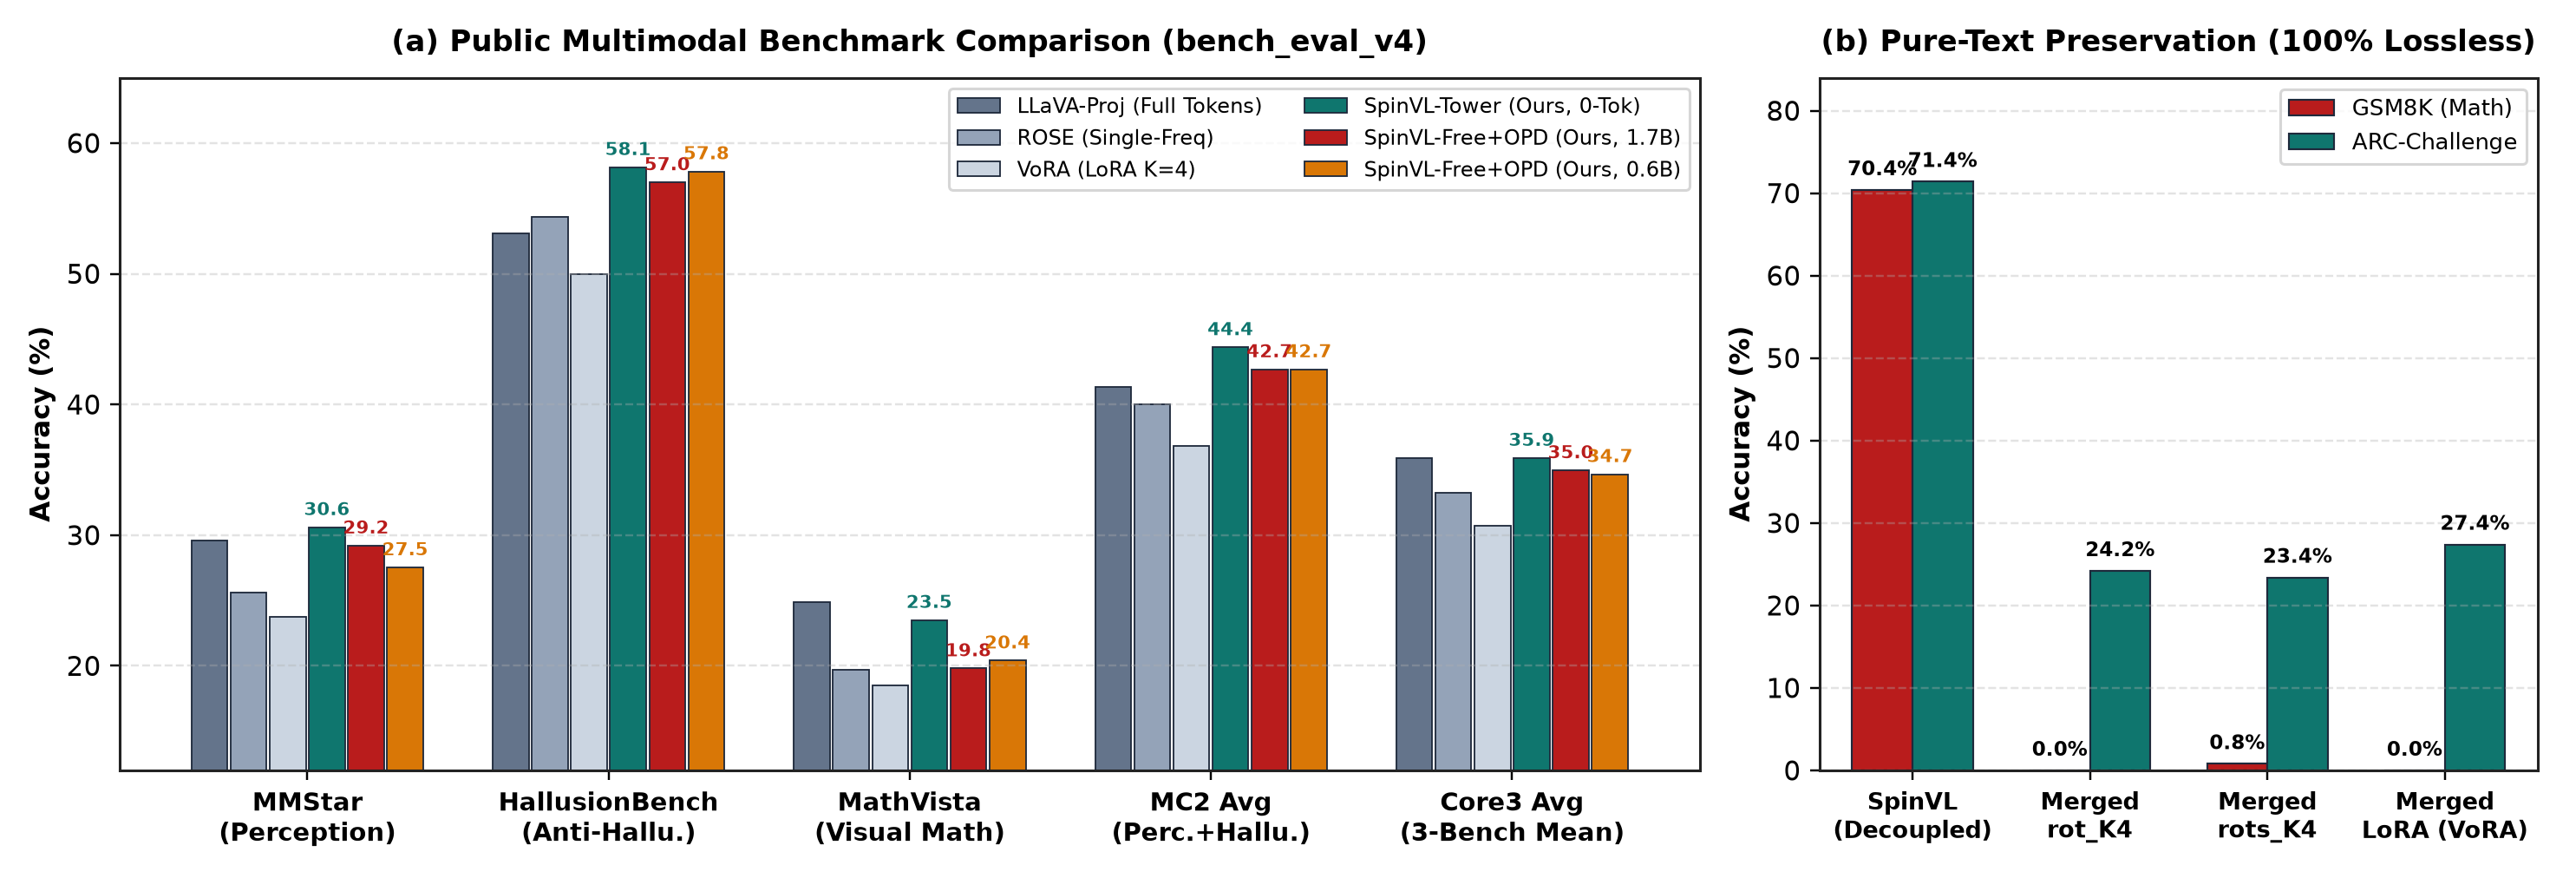
\includegraphics[width=0.96\textwidth]{fig_main_results.png}
\caption{\textbf{(a) Main public benchmark comparison} ($1.7$B student,
within-mixture comparisons at $s{=}0$, plus $0.6$B tower-free). \modelname{}
leads on perception (MMStar) and anti-hallucination (HallusionBench) while
keeping the backbone free of visual tokens; the tower-free variant matches or
exceeds full-token LLaVA on MC2 at a quarter of its compute. \textbf{(b)
Pure-text retention.} Only the decoupled pathway preserves GSM8K ($70.4\%$) and
ARC-C ($71.4\%$); permanently merging vision adapters---LoRA, rotation, or
rotation with scaling---collapses mathematical reasoning.}
\label{fig:mainres}
\end{figure*}

Tab.~\ref{tab:main} and Fig.~\ref{fig:mainres} summarise the comparison.
Four observations follow.

\emph{(i) Within the same mixture, perception and anti-hallucination scores
exceed token concatenation without any visual token.} On the $21$k base mixture
($s{=}0$), \modelname-Tower with the hybrid generator reaches $30.60\%$ on
MMStar and $58.15\%$ on HallusionBench, against $29.60\%$ and $53.10\%$ for the
retrained token-concatenation baseline. The MC2 aggregate rises from $41.35\%$
to $44.37\%$ ($+3.02$ points) and Core3 reaches $35.75\%$ against $35.87\%$
($99.7\%$), while the backbone processes text of length $T$ rather than $T+N$
in every one of its $28$ layers.

\emph{(ii) Diagram reasoning catches up on the $+open$ mixture with genuine
visual grounding.} On the $28$k +open mixture ($s{=}0$), the multi-frequency
generator with on-policy distillation reaches $23.50\%$ on MathVista ($+4.10$
points above its shuffled-image control at $19.40\%$ and $+4.90$ above blank at
$18.60\%$), bringing Core3 to $35.90\%$ against $36.14\%$ ($99.3\%$) for the
$28$k token-concatenation baseline and $36.01\%$ for $32$-token spatial pooling.

\emph{(iii) Removing the encoder costs little compute and preserves parity on
MC2.} With no external vision tower at all, \modelname-Free{} (\texttt{rots}
$K{=}4$ + \texttt{mf}) reaches $41.32\%$ MC2 on the $21$k base mixture (vs.\
$36.84\%$ for VoRA~\citep{vora2025} under the identical \texttt{mf} deep tier
and \texttt{ce} arm), and adding VL-OPD on the base mixture lifts
\modelname-Free{} (\texttt{hyb}) from $40.21\%$ to $42.46\%$ MC2 and from
$33.57\%$ to $34.91\%$ Core3 ($97.3\%$ of the $21$k LLaVA baseline's Core3)
while using $74.2\%$ fewer FLOPs.

\emph{(iv) Both tiers contribute when held under strict single-factor controls.}
Holding the deep tier fixed at \texttt{mf} and comparing frontends in the same
\texttt{ce} arm ($21$k base, $s{=}0$), rotation with scaling (\texttt{rots})
beats rank-$16$ LoRA by $+4.48$ points of MC2 ($41.32\%$ vs.\ $36.84\%$) and
$+2.82$ points of Core3 ($33.55\%$ vs.\ $30.73\%$) with $36\%$ fewer frontend
parameters ($2.40$M vs.\ $3.74$M); under a single-frequency deep tier,
\texttt{rots} still leads LoRA ($38.14\%$ vs.\ $36.84\%$ MC2). Holding the
frontend fixed (external encoder, $21$k base, $s{=}0$) and comparing deep
generators, multi-frequency and hybrid rotation beat single-frequency ROSE by
$+0.75$ and $+4.39$ points of MC2 ($40.73\%$ and $44.37\%$ vs.\ $39.98\%$).

\subsection{Scaling Across Student Sizes and Seeds}
\label{sec:scaling}

\begin{table}[t]
\centering
\caption{\textbf{Cross-size behaviour and seed variance} (public benchmarks).
$0.6$B models are competitive with $1.7$B baselines on perception; $8$B
students do not benefit, since the frozen backbone is not the bottleneck.
All single-run rows use $s{=}0$, and $3$-seed rows average $s\in\{0,1,2\}$. Error bars are sample standard deviations ($\mathrm{ddof}{=}1$).}
\label{tab:scale}
\footnotesize
\setlength{\tabcolsep}{2.4pt}
\resizebox{\columnwidth}{!}{%
\begin{tabular}{@{}llcccccc@{}}
\toprule
Scale & Model (Mix, Seed) & MMStar & Hallu. & MathV. & MC2 & Core3 & Avg6 \\
\midrule
$0.6$B & Tower (\texttt{hyb}, $28$k, $s{=}0$)    & 26.40 & 57.73 & 20.20 & 42.06 & 34.78 & 17.97 \\
$0.6$B & Free (CE, $21$k, $s{=}0$)               & 28.07 & 54.68 & 20.40 & 41.37 & 34.38 & 18.03 \\
$0.6$B & Free+OPD ($21$k, $s{=}0$)               & 28.87 & 54.47 & 19.00 & 41.67 & 34.11 & 17.69 \\
$0.6$B & Free+OPD ($28$k, $s{=}0$)               & 27.53 & 57.83 & 18.60 & \textbf{42.68} & \textbf{34.66} & \textbf{18.05} \\
$0.6$B & Free+OPD ($28$k, $3$ seeds)             & 25.36$_{\pm2.70}$ & \textbf{57.69}$_{\pm0.12}$ & 18.73$_{\pm0.12}$ & 41.52$_{\pm1.39}$ & 33.93$_{\pm0.90}$ & 17.62$_{\pm0.51}$ \\
\midrule
$1.7$B & Tower (\texttt{hyb}, $28$k, $3$ seeds)  & 26.56$_{\pm1.49}$ & 56.36$_{\pm1.04}$ & 18.97$_{\pm1.18}$ & \textbf{41.46}$_{\pm0.75}$ & \textbf{33.96}$_{\pm0.59}$ & \textbf{17.68}$_{\pm0.43}$ \\
$1.7$B & Free (\texttt{hyb}, $28$k, $3$ seeds)   & \textbf{26.89}$_{\pm2.28}$ & 53.84$_{\pm1.27}$ & 19.00$_{\pm2.05}$ & 40.36$_{\pm0.83}$ & 33.24$_{\pm1.14}$ & 17.27$_{\pm0.44}$ \\
$1.7$B & Free+OPD ($28$k, $3$ seeds)             & 26.11$_{\pm3.21}$ & 56.12$_{\pm1.74}$ & \textbf{19.13}$_{\pm1.00}$ & 41.11$_{\pm1.35}$ & 33.79$_{\pm1.05}$ & 17.49$_{\pm0.30}$ \\
\midrule
$8$B   & Tower (\texttt{hyb}, $28$k, $s{=}0$)    & 25.67 & 54.15 & 19.90 & 39.91 & 33.24 & 17.30 \\
$8$B   & Free (\texttt{hyb}, $28$k, $s{=}0$)     & 24.80 & \textbf{56.99} & 19.20 & \textbf{40.90} & \textbf{33.66} & \textbf{17.50} \\
$8$B   & Free+OPD ($28$k, $s{=}0$)               & \textbf{27.40} & 53.31 & 18.10 & 40.36 & 32.94 & 16.91 \\
\bottomrule
\end{tabular}}
\end{table}

Tab.~\ref{tab:scale} reports the same pipelines with $0.6$B and $8$B students,
as well as three-seed averages ($s\in\{0,1,2\}$) on the $28$k +open mixture.
A $0.6$B tower-free model reaches $42.68\%$ MC2 at $s{=}0$ ($41.52\%{\pm}1.39\%$
across three seeds), matching the $1.7$B models on perception and
hallucination; the smallest student is therefore already sufficient for the
abilities this paradigm provides. On $1.7$B (+open, $3$ seeds), online
distillation improves the tower-free model's three-seed mean from $40.36\%$ to
$41.11\%$ MC2 ($+0.75$ points) and from $33.24\%$ to $33.79\%$ Core3. Scaling
to $8$B does not help, and in our measurements slightly hurts: because the
backbone is frozen and only the rotation generators are trained, additional
capacity in the LLM does not translate into better visual steering, while a
larger model makes optimisation of the small adapter set harder at a fixed step
budget. We see this as evidence that the bottleneck is the interface, not the
language model.

\subsection{Ablations}
\label{sec:abl}

\begin{figure*}[t]
\centering
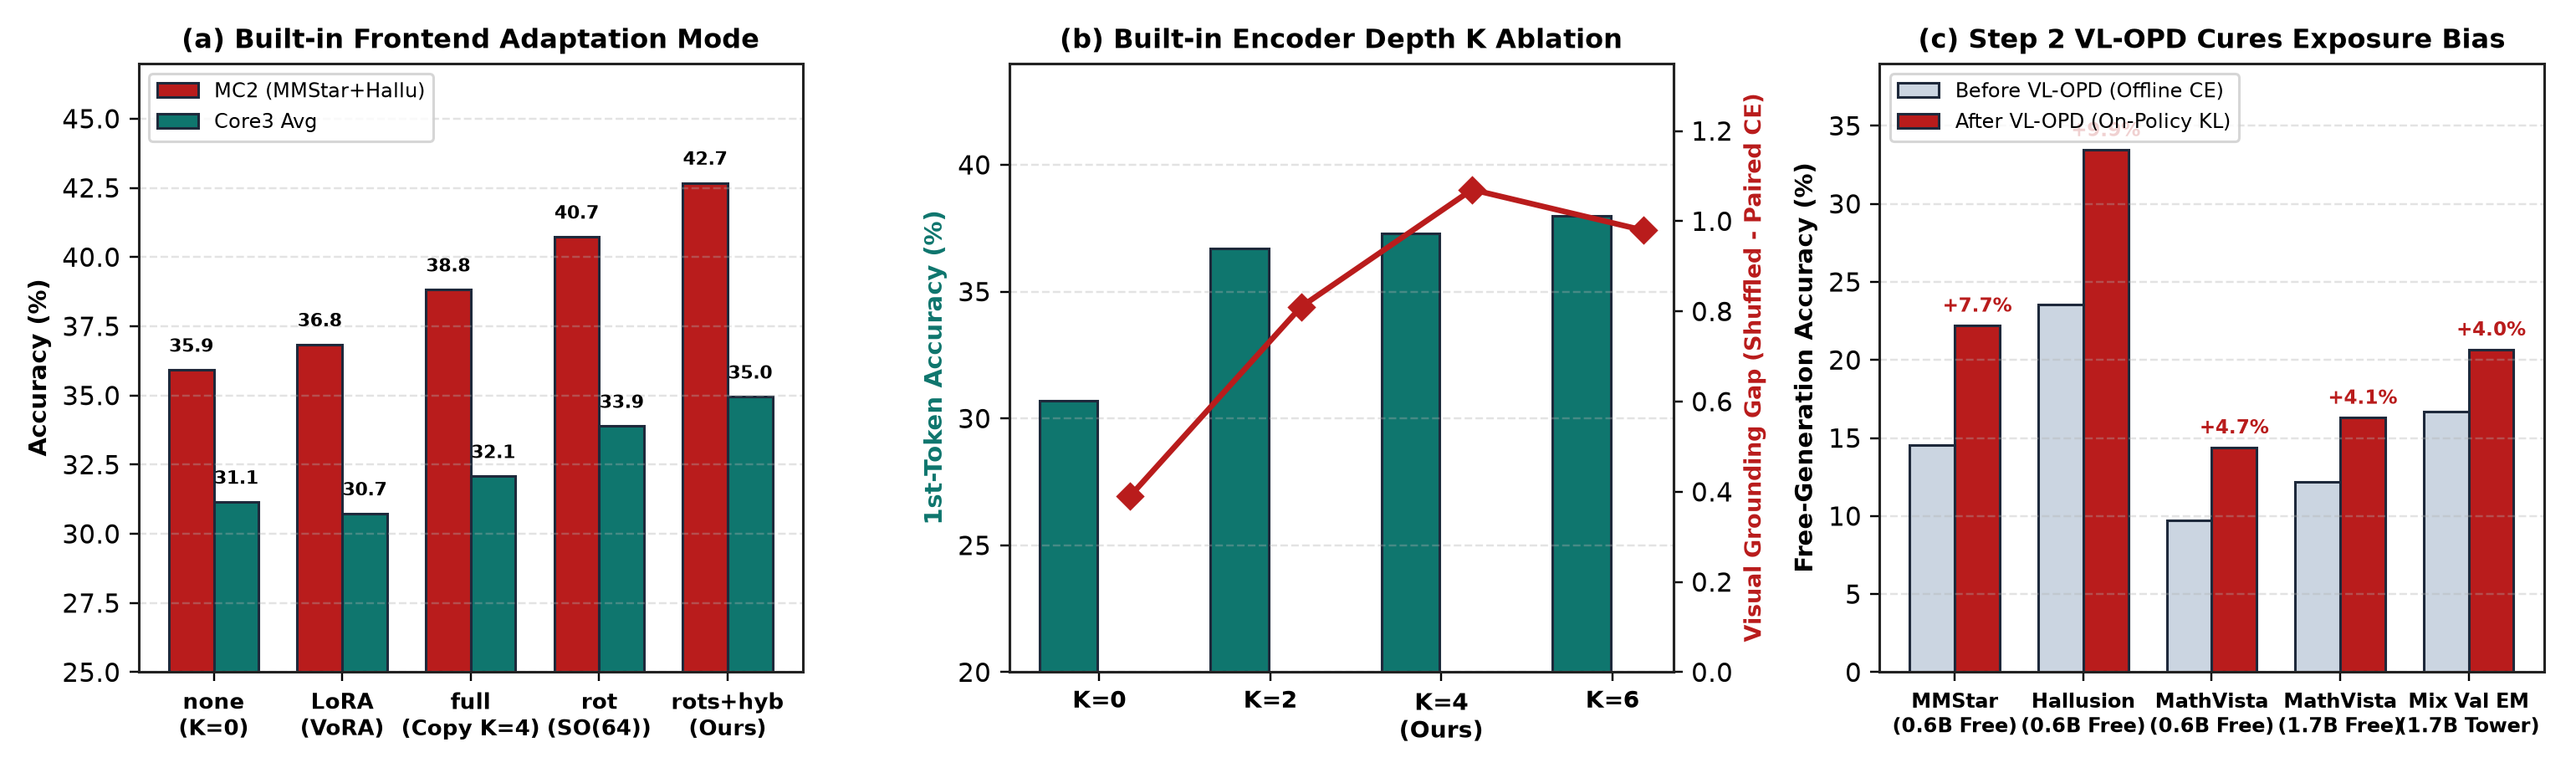
\includegraphics[width=0.98\textwidth]{fig_ablations.png}
\caption{\textbf{Ablation studies.} \textbf{(a)} Built-in frontend
parameterisation grouped by initialisation arm (\texttt{rel} vs.\ \texttt{ce}).
\textbf{(b)} Built-in encoder depth $K\in\{0,2,4,6\}$, showing validation
first-token accuracy and visual grounding gap (shuffled minus paired CE).
\textbf{(c)} Step~2 online policy distillation (\texttt{VL-OPD}) gains under
forced free-form greedy generation.}
\label{fig:abl}
\end{figure*}

\begin{table}[t]
\centering
\caption{\textbf{Frontend parameterisation on the $21$k base mixture ($s{=}0$).}
Every row is reported from a single joint checkpoint and its exact public
benchmark evaluation. Rows are grouped by initialisation arm (\texttt{rel} vs.\
\texttt{ce}) and deep rotation tier (\texttt{single}, \texttt{mf}, \texttt{hyb}).
``Val CE'', ``Gap'' (shuffled minus paired CE), and ``1st/Full'' are measured on
the held-out validation split.}
\label{tab:front}
\footnotesize
\setlength{\tabcolsep}{2.2pt}
\resizebox{\columnwidth}{!}{%
\begin{tabular}{@{}lllccccccc@{}}
\toprule
Frontend & Arm & Deep & Params & Val CE$\downarrow$ & Gap$\uparrow$ & 1st/Full & MC2$\uparrow$ & Core3$\uparrow$ & Avg6$\uparrow$ \\
\midrule
none ($K{=}0$)     & rel & single & 0     & 5.237 & 0.501 & 24.0/16.0 & 35.92 & 31.15 & 15.81 \\
rot                & rel & single & 2.32M & 1.973 & 1.130 & 40.7/17.3 & \textbf{40.73} & \textbf{33.89} & \textbf{17.55} \\
full copy          & rel & single & 201M  & 1.745 & 1.857 & 43.3/20.0 & 38.82 & 32.08 & 16.80 \\
\midrule
\textbf{\texttt{rots}} & ce & single & \textbf{2.40M} & 2.019 & 0.850 & 42.0/18.7 & \textbf{38.14} & \textbf{31.32} & \textbf{16.12} \\
\midrule
LoRA ($r{=}16$)    & ce  & mf     & 3.74M & 1.532 & 1.667 & 44.7/18.7 & 36.84 & 30.73 & 15.82 \\
\textbf{\texttt{rots}} & ce & mf  & \textbf{2.40M} & 1.549 & \textbf{1.783} & 43.3/17.3 & \textbf{41.32} & \textbf{33.55} & \textbf{17.33} \\
\textbf{\texttt{rots}} & ce & hyb & \textbf{2.40M} & 1.554 & \textbf{1.866} & 43.3/16.0 & 40.20 & \textbf{33.57} & \textbf{17.37} \\
\bottomrule
\end{tabular}}
\end{table}

\paragraph{Frontend parameterisation (Sec.~\ref{sec:abl}).}
Tab.~\ref{tab:front} and Fig.~\ref{fig:abl}(a) isolate the ways of turning the
first $K{=}4$ layers into a vision encoder on the $21$k base mixture ($s{=}0$),
with every row's validation and public metrics taken from the exact same
checkpoint. Within the \texttt{rel}-initialised single-frequency group, pure
rotation (\texttt{rot}) reaches $40.73\%$ MC2 and $17.55\%$ Avg6 with $2.32$M
in-layer parameters, ahead of copying the layers ($38.82\%$, $201$M) and of dropping the
layers entirely ($35.92\%$, $K{=}0$). Within the \texttt{ce}-initialised group,
holding the deep tier fixed at \texttt{mf}, rotation with channel scaling
(\texttt{rots}) beats rank-$16$ LoRA by $+4.48$ points of MC2 ($41.32\%$ vs.\
$36.84\%$), $+2.82$ points of Core3 ($33.55\%$ vs.\ $30.73\%$), and a larger
validation grounding gap ($1.783$ vs.\ $1.667$). Even with a single-frequency deep
tier, \texttt{rots} ($38.14\%$ MC2) exceeds LoRA+\texttt{mf} ($36.84\%$).
(Note: in this $21$k sweep the LoRA baseline used transposed output-projection
ranks totaling $3.74$M static parameters; in our $44$k debiased implementation
of Tab.~\ref{tab:grounding}, rank-$16$ LoRA uses $2.49$M static parameters
against $2.40$M for \texttt{rots}, plus the shared $54.03$M patch-embedding and
merger module.)

\paragraph{Depth of the built-in encoder.}
\begin{table}[t]
\centering
\caption{\textbf{Frontend depth} on the $28$k \emph{+open} mixture (\texttt{hyb}
deep tier). Every row comes from a single joint checkpoint ($s{=}0$, plus the
$3$-seed mean at $K{=}4$). Grounding gap is the cross-entropy difference
between shuffled and correctly paired validation images.}
\label{tab:depth}
\footnotesize
\setlength{\tabcolsep}{3.0pt}
\resizebox{\columnwidth}{!}{%
\begin{tabular}{@{}lccccccc@{}}
\toprule
$K$ & Params & CE$\downarrow$ & Gap$\uparrow$ & 1st$\uparrow$ & MC2 & Core3 & Avg6 \\
\midrule
$0$ ($s{=}0$)         & 0      & 2.382 & 0.387 & 30.7 & 42.31 & 34.61 & 17.94 \\
$2$ ($s{=}0$)         & 1.20M  & \textbf{2.267} & 0.815 & 36.7 & 41.30 & 33.93 & 17.68 \\
\textbf{$4$ ($s{=}0$)} & \textbf{2.40M} & 2.294 & \underline{0.896} & 36.0 & 41.09 & 33.76 & 17.58 \\
\textbf{$4$ ($3$ seeds)} & \textbf{2.40M} & 2.329 & \textbf{1.150} & 35.8 & 40.36 & 33.24 & 17.27 \\
$6$ ($s{=}0$)         & 3.59M  & 2.272 & 0.978 & \textbf{38.0} & 41.94 & 33.90 & 17.66 \\
\bottomrule
\end{tabular}}
\end{table}
Tab.~\ref{tab:depth} varies $K$ on the $28$k +open mixture. On the validation
split, the visual grounding gap rises sharply from $0.387$ at $K{=}0$ to $0.896$
at $K{=}4$ ($s{=}0$; $1.150$ across three seeds) and $0.978$ at $K{=}6$, while
first-token accuracy rises from $30.7\%$ to $36.0\%$--$38.0\%$. Thus four early
LLM layers more than double the model's sensitivity to the paired image on the
training distribution, whereas zero-shot public MC2 stays in a narrow band
($41.09\%$--$42.31\%$ at $s{=}0$). We therefore fix $K{=}4$ as the default
trade-off between visual conditioning and compute.

\paragraph{On-policy distillation and feature supervision.}
\begin{table}[t]
\centering
\caption{\textbf{Step~2 online distillation comparison and free-generation gains.}
Top: comparison of external sequence/on-policy distillation objectives from the
same \modelname-Free ($1.7$B) checkpoint ($500$ steps). Bottom: free-form
greedy generation accuracy with candidate scoring disabled.}
\label{tab:opd}
\footnotesize
\setlength{\tabcolsep}{2.8pt}
\resizebox{\columnwidth}{!}{%
\begin{tabular}{@{}llcccc@{}}
\toprule
Objective / Pair & Split / Mode & Val CE$\downarrow$ & EOS$\uparrow$ & MC2$\uparrow$ & Core3$\uparrow$ \\
\midrule
Offline CE (Start)            & teacher-forced & 2.294 & 100.0\% & 41.09 & 33.76 \\
+ GKD~\citep{agarwal2024gkd}  & JSD ($\beta{=}0.5$) & 2.301 & \textbf{99.0\%} & 38.79 & 32.46 \\
+ MiniLLM~\citep{gu2024minillm} & Reverse KL   & 2.565 & 59.0\% & 40.46 & 32.34 \\
+ SeqKD~\citep{kim2016sequence} & Hard Top-$1$ & 2.417 & 84.0\% & \textbf{41.11} & \textbf{33.50} \\
+ VL-OPD (Ours)               & Forward KL      & 2.475 & 95.0\% & \underline{40.35} & \underline{32.90} \\
\midrule
\multicolumn{2}{@{}l}{\textit{Free-form greedy generation}} & MMStar & Hallu. & MathV. & MC2 \\
$0.6$B Free ($28$k) & before VL-OPD & 14.53 & 23.55 & 9.70 & 19.04 \\
            & after VL-OPD  & \textbf{22.20} & \textbf{33.44} & \textbf{14.40} & \textbf{27.82} \\
$1.7$B Free ($21$k) & before VL-OPD & 14.07 & 24.40 & 8.30 & 19.23 \\
            & after VL-OPD  & \textbf{18.13} & 22.92 & \textbf{9.30} & \textbf{20.53} \\
\bottomrule
\end{tabular}}
\end{table}

Tab.~\ref{tab:opd} compares our forward-KL \texttt{VL-OPD} against three
established sequence and on-policy distillation objectives, all starting from
the \emph{same} \modelname-Free ($1.7$B, \emph{+open}, seed $0$) checkpoint and
trained for $500$ steps. We report this comparison in full, including where our
objective loses. On candidate-scoring aggregates \texttt{VL-OPD} does
\emph{not} beat the alternatives: it reaches $40.35\%$ MC2 and $32.90\%$ Core3,
below SeqKD ($41.11/33.50$) and below the offline starting checkpoint itself
($41.09/33.76$). End-of-sequence termination likewise \emph{degrades} from
$100\%$ at the start to $95\%$ under forward KL, although it degrades far less
than under mode-seeking reverse KL (MiniLLM~\citep{gu2024minillm}, $59\%$),
which locks onto a single mode and amplifies repetitive run-on tails. The
grounding gap (shuffled minus paired validation CE) also shrinks under
\texttt{VL-OPD}, from $0.896$ to $0.674$, i.e.\ distillation at this scale makes
the model \emph{less} image-dependent on the training distribution, not more.
The one place \texttt{VL-OPD} helps unambiguously is forced free-form decoding
on the $0.6$B tower-free model, where it adds $+7.67$ points on MMStar, $+9.89$
on HallusionBench and $+4.70$ on MathVista; on the $1.7$B model the HallusionBench
free-form score instead \emph{falls} by $1.48$ points
(Tab.~\ref{tab:opd}, bottom). We therefore claim only that forward KL is a
stable terminator relative to reverse KL and that it improves small-model
free-form generation, not that it dominates other distillation objectives.
Finally, switching off the feature term of Eq.~\eqref{eq:feat} during joint
training yields $42.63\%$ MC2 and $34.89\%$ Core3 against the supervised
variant's $41.09\%$ and $33.76\%$ at the same starting point: removing feature
alignment does not hurt, and slightly helps, the public aggregates.

\subsection{Efficiency and Text Retention}
\label{sec:eff}

\begin{table}[t]
\centering
\caption{\textbf{Compute and latency} at increasing image resolution
($1.7$B, text query length $64$). Latency is measured with the GPU
exclusively occupied. At $4096$ patches \modelname{} needs $74.2\%$ fewer
FLOPs and is $19.5\%$ faster than token concatenation.}
\label{tab:eff}
\footnotesize
\setlength{\tabcolsep}{4pt}
\begin{tabular}{@{}rcccc@{}}
\toprule
Patches & \modelname{} & ROSE & LLaVA & Saving \\
 & (TFLOPs/ms) & (TFLOPs/ms) & (TFLOPs/ms) & FLOPs \\
\midrule
256  & 0.30/65.8  & 0.47/58.2  & 0.66/25.7  & $-54.8\%$ \\
576  & 0.45/66.6  & 0.86/57.8  & 1.27/25.6  & $-64.9\%$ \\
1024 & 0.67/69.8  & 1.45/63.8  & 2.18/33.7  & $-69.4\%$ \\
2304 & 1.37/80.4  & 3.40/86.0  & 5.07/66.9  & $-72.9\%$ \\
4096 & \textbf{2.54/99.4} & 6.82/126.1 & \textbf{9.85}/123.4 & $\mathbf{-74.2\%}$ \\
\bottomrule
\end{tabular}
\end{table}

\begin{figure*}[t]
\centering
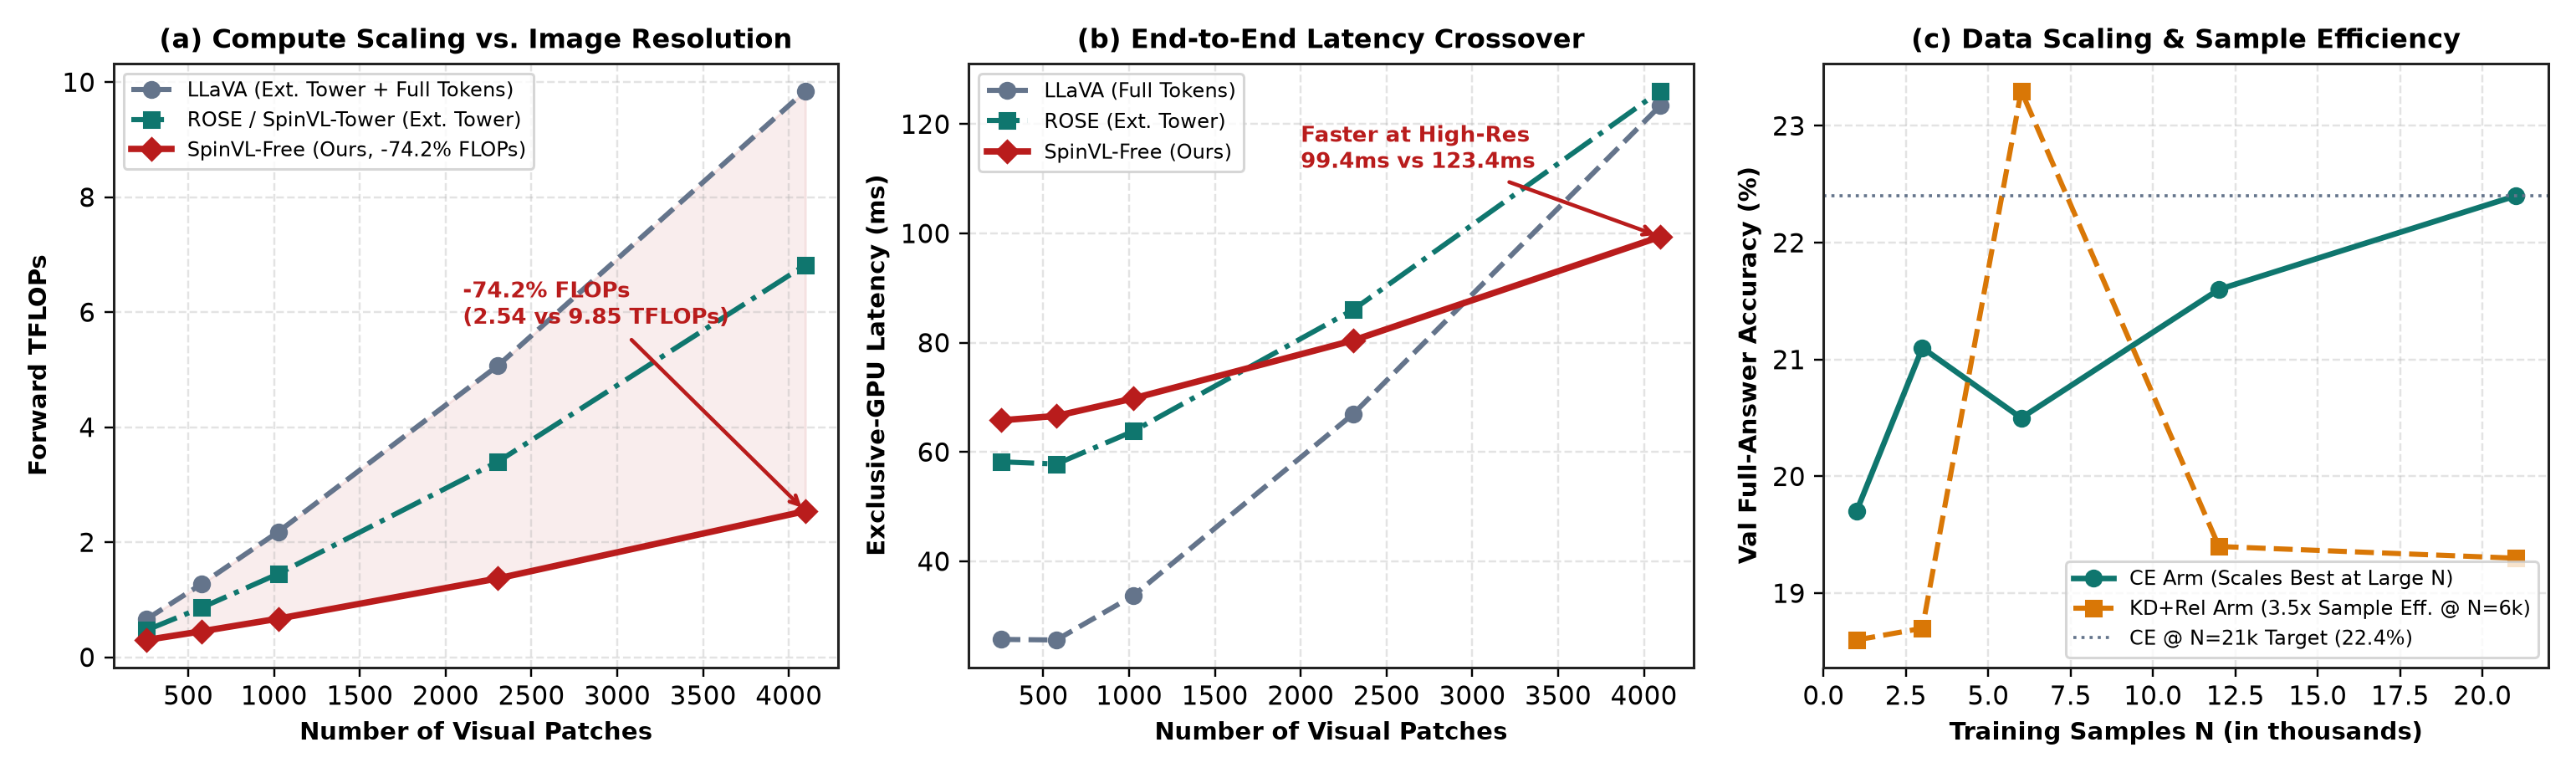
\includegraphics[width=0.98\textwidth]{fig_efficiency.png}
\caption{\textbf{Efficiency and data scaling.} \textbf{(a, b)} Forward compute
(TFLOPs) and exclusive-GPU latency versus visual patch count; discarding image
tokens after layer $K{=}4$ saves $74.2\%$ FLOPs at $4096$ patches and crosses
over in wall-clock latency beyond ${\sim}3$k patches. \textbf{(c)} Validation
full-answer accuracy versus training sample size $N\in\{1\text{k}\dots21\text{k}\}$:
distillation (\texttt{KD+Rel}) achieves $3.5\times$ sample efficiency at
$N{=}6$k, while the \texttt{CE} arm scales best at full data.}
\label{fig:eff}
\end{figure*}

Tab.~\ref{tab:eff} and Fig.~\ref{fig:eff} quantify the trade-off. The saving
grows with resolution because the baseline pays $O((T+N)^2)$ in every layer
while \modelname{} pays $O(N^2)$ once for $K$ layers. Up to $2{,}304$ patches
the baseline is still faster in wall-clock terms on our hardware ($66.9$ vs.\
$80.4$ ms), since the frontend's bidirectional pass over all patches is not
free; between $2{,}304$ and $4{,}096$ patches (${\sim}3$k patches) the ordering
reverses and at $4{,}096$ patches \modelname{} is $19.5\%$ faster ($99.4$ vs.\
$123.4$ ms).

Text retention is reported in Fig.~\ref{fig:mainres} (right). The decoupled
pathway keeps GSM8K at $70.4\%$ and ARC-C at $71.4\%$, identical to the
unmodified LLM. Merging the frontend into the text layers---whether as LoRA,
pure rotation, or rotation with scaling (using the exact post-multiplied form
$W\mathrm{diag}(d)R_{\mathrm{s}}^{\top}$)---drops GSM8K to $0.0\%$, $0.0\%$ and
$0.8\%$ respectively. This is the clearest argument for keeping vision
adapters context-gated instead of permanently fused.

\subsection{Where the Paradigm Stops: Boundary and Grounding Diagnostics}
\label{sec:boundary}

\begin{table}[t]
\centering
\caption{\textbf{Format boundary study.} Adding $8{,}334$ open-ended
document/chart questions and $2{,}101$ geometry problems to the training
mixture ($21$k$\to$$28$k, $s{=}0$). Geometry doubles for \modelname{}, whereas
character-level chart reading and scene text stay flat for both methods: the
residual gap is architectural, not a data artefact.}
\label{tab:boundary}
\footnotesize
\setlength{\tabcolsep}{4pt}
\begin{tabular}{@{}llccc@{}}
\toprule
Mixture & Model & ChartQA & OCRBench & Geo3K \\
\midrule
base ($21$k)      & LLaVA-Proj & \textbf{10.40} & \textbf{1.60} & \textbf{6.49} \\
base ($21$k)      & \modelname-Tower & 1.08 & 0.00 & 1.83 \\
\midrule
+open ($28$k)     & LLaVA-Proj & \textbf{10.32} & \textbf{1.10} & 5.49 \\
+open ($28$k)     & \modelname-Tower & 1.24 & 0.00 & \textbf{3.83} \\
\bottomrule
\end{tabular}
\end{table}

\begin{table}[t]
\centering
\caption{\textbf{Debiased $44$k mixture under unified frozen-backbone auditing}
($s{=}0$). All methods are trained on the identical $44$k deduplicated,
label-balanced mixture ($1{:}1$ Yes/No, $1{:}1{:}1{:}1$ A/B/C/D, image-grouped
split) with the LLM $100\%$ frozen, unified greedy decoding, and official
relaxed ChartQA scoring. ``Val CE/EM'' and ``Gap'' (shuffled minus paired CE)
are measured on the held-out validation split.}
\label{tab:grounding}
\footnotesize
\setlength{\tabcolsep}{1.8pt}
\resizebox{\columnwidth}{!}{%
\begin{tabular}{@{}lccccccccc@{}}
\toprule
Model ($44$k Debiased, $s{=}0$) & Val CE/EM & Gap$\uparrow$ & MMStar & Hallu. & MathV. & ChartQA & MC2 & Core3 & Avg6 \\
\midrule
LLaVA-Proj (Full Tok.)         & --- & --- & 28.60 & 52.05 & \textbf{25.70} & \textbf{10.52} & 40.33 & \textbf{35.45} & \textbf{20.77} \\
\midrule
ROSE (Single-Freq Rot.)        & 2.235/21.6\% & \textbf{1.345} & 26.07 & 48.16 & 18.40 & 0.72 & 37.11 & 30.88 & 15.70 \\
CA-Only ($R_{\ell}{\equiv}I$)  & 1.197/\textbf{41.2\%} & 0.187 & 28.27 & 52.16 & \textbf{23.90} & 9.44 & 40.21 & 34.77 & 19.59 \\
\textbf{\modelname-Tower (\texttt{srot}, $R_1$)} & 1.186/40.3\% & 0.239 & 28.20 & 53.21 & 23.30 & 9.04 & 40.70 & 34.90 & 19.63 \\
\textbf{\modelname-Tower (\texttt{mf}, $R_2$)}   & 1.189/40.5\% & 0.212 & \textbf{28.73} & \textbf{54.68} & 22.90 & 9.36 & \textbf{41.71} & \textbf{35.44} & \textbf{20.18} \\
\textbf{\modelname-Tower (\texttt{mf+qc}, $R_3$)} & \textbf{1.186}/39.5\% & 0.230 & 28.40 & 53.94 & 22.80 & \textbf{9.52} & 41.17 & 35.05 & 19.92 \\
\midrule
Patch-Merger ($K{=}0$, $S_0$)                    & 1.181/40.1\% & 0.068 & 27.67 & 52.16 & 22.90 & 9.44 & 39.91 & 34.24 & 19.58 \\
VoRA (LoRA $K{=}4$, $S_1$)                       & 1.163/40.3\% & 0.149 & 27.93 & 51.00 & 23.30 & 9.04 & 39.47 & 34.08 & 19.23 \\
\textbf{\modelname-Free (\texttt{rots}+CA, $F_2$)} & 1.835/26.4\% & 0.092 & 27.60 & \textbf{53.31} & 23.50 & 7.96 & 40.46 & 34.80 & 19.31 \\
\textbf{\modelname-Free (\texttt{rots}+\texttt{mf}, $S_2$)} & \textbf{1.155}/40.8\% & 0.152 & 28.87 & 49.42 & 23.60 & 9.44 & 39.14 & 33.96 & 19.29 \\
\textbf{+ Step 2 Cont.\ CE ($M_0$)}              & \textbf{1.155}/\textbf{41.2\%} & \textbf{0.192} & \textbf{29.40} & 52.47 & 23.50 & \textbf{9.88} & \textbf{40.94} & 35.12 & 19.99 \\
\textbf{+ Step 2 Off-Policy KD ($M_1$)}          & 1.229/39.9\% & 0.156 & 29.07 & \textbf{52.68} & 24.20 & 9.68 & 40.87 & \textbf{35.32} & \textbf{20.08} \\
\textbf{+ Step 2 Fwd-KL VL-OPD ($M_2$)}          & 1.233/40.8\% & 0.149 & 28.73 & 52.05 & \textbf{24.90} & 9.44 & 40.39 & 35.23 & 20.00 \\
\textbf{+ Step 2 JSD VL-OPD ($M_3$)}             & \textbf{1.154}/40.8\% & 0.181 & 28.60 & \textbf{52.68} & 23.50 & 9.64 & 40.64 & 34.93 & 19.85 \\
\bottomrule
\end{tabular}}
\end{table}

Our benchmarks mix two very different demands. Perception, hallucination and
diagram reasoning ask \emph{what is in the image}; chart reading and OCR ask
the model to \emph{copy a string exactly}. To separate the two we first audited
the base mixture and found that it contains no open-ended chart item and no
scene-text item at all: the chart-like portion is entirely multiple choice.
We therefore rebuilt the mixture to include the missing formats and retrained
both the token-concatenation baseline and \modelname{} on it
(Tab.~\ref{tab:boundary}). Two results are decisive. First, the baseline's
ChartQA accuracy does not move ($10.40\%\to10.32\%$) and its OCRBench accuracy
falls ($1.60\%\to1.10\%$), even though $6{,}500$ document and chart questions
were added: exact copying is not a data problem for the baseline, it is a
capability it already has and the added data does not improve. Second,
\modelname{}'s geometry accuracy doubles ($1.83\%\to3.83\%$), so the added data
is being used where the architecture supports the task. Operator-level
modulation compresses the image into rotation parameters; it cannot maintain a
per-character key-value memory, so copying a five-digit axis label fails for
structural rather than statistical reasons.

Finally, to disentangle genuine visual grounding from label-prior adaptation
and verify every design choice under strict frozen-backbone auditing, we
evaluated all three tiers on the $44$k debiased mixture with unified greedy
decoding and zero-shot relaxed ChartQA scoring (Tab.~\ref{tab:grounding}). Three
positive conclusions follow. First, restricting dynamic rotations to the five
residual-stream entry projections with Lie-algebra tangent bounding
($\tau_{\mathrm{rot}}{=}0.12$) eliminates the decoding instability of unbounded
rotations: \modelname-Tower progresses monotonically from single-frequency
rotation ($R_1$: $19.63\%$ Avg6, $40.70\%$ MC2) to multi-frequency rotation
($R_2$: $20.18\%$ Avg6, $41.71\%$ MC2, $35.44\%$ Core3) and question-conditioned
multi-frequency rotation ($R_3$: $9.52\%$ ChartQA, $0.70\%$ OCRBench; $20.28\%$
Avg6 at $s{=}1$), outperforming both single-frequency ROSE ($15.70\%$ Avg6,
$37.11\%$ MC2) and cross-attention alone ($19.59\%$ Avg6, $40.21\%$ MC2), while
restoring free-form generation from $11.79\%$ to $40.89\%$--$41.67\%$ MC2
($99.9\%$--$100.0\%$ EOS termination). Second, combining the shallow \texttt{rots}
($K{=}4$) frontend with bounded multi-frequency rotation yields a large
synergistic gain over pairing \texttt{rots} with cross-attention alone: validation
CE drops from $1.835$ to $1.155$, validation $1{,}000$-item exact match jumps
from $26.4\%$ to $40.8\%$, and the grounding gap expands $2.24\times$ over
$K{=}0$ ($0.152$ vs.\ $0.068$ nats), while outperforming $K{=}4$ LoRA ($S_1$)
across validation CE, gap, exact match, and public MMStar ($28.87\%$ vs.\
$27.93\%$). At $4{,}096$ patches, skipping $\text{down}/\text{out}$ rotations
further lowers \modelname-Free{} prefill latency to $101.9$\,ms ($20.0\%$ faster
than LLaVA-Proj's $127.2$\,ms) and compute to $2.67$ TFLOPs ($-72.5\%$). Third,
Step~2 distillation on top of \modelname-Free{} ($S_2$) pushes the tower-free
model to $20.08\%$ Avg6 and $35.32\%$ Core3 ($M_1$, $99.6\%$ of $44$k
full-token LLaVA-Proj's $35.45\%$ Core3) and $40.94\%$ MC2 ($M_0$, above
LLaVA-Proj's $40.33\%$), while on-policy forward-KL VL-OPD ($M_2$) preserves
$40.8\%$ validation exact match (vs.\ $39.9\%$ for off-policy KD) and achieves
the highest tower-free MathVista accuracy ($24.90\%$, $+1.40$ over $M_0$). On
MMStar, cross-image shuffle deltas remain small across all frozen-backbone
models at this $44$k scale (including LLaVA-Proj: $28.60\%$ real vs.\ $28.00\%$
shuffled), confirming that web-scale pretraining is needed for strong zero-shot
spatial sensitivity across every open category.

\section{Limitations and Conclusion}
\label{sec:conclusion}

\paragraph{Limitations.}
We state four limits explicitly, because they define the regime in which the
claims hold.

\emph{Dense transcription remains out of reach.} As shown in
Sec.~\ref{sec:boundary}, exact character copying (chart axis labels, receipts,
handwritten formulae) does not follow from operator-level modulation, and the
data study we ran---retraining a token-concatenation baseline on identical
data---indicates that the gap is architectural rather than a data artefact. A
practical extension is to retain a small number of pooled visual tokens for
this class of queries only; we deliberately do not include such a variant here,
because it would break the zero-token property that the paper is about.

\emph{The backbone is never adapted.} Keeping the LLM frozen is what buys
bit-exact text retention and cheap training, but it also caps the achievable
accuracy: a $8$B student is no better than a $0.6$B one in our measurements,
which suggests that the adapter interface, not the language capacity, is the
bottleneck. Allowing even a low-rank update of the backbone would likely raise
the ceiling, at the cost of the lossless property.

\emph{Training scale is modest.} Our mixtures contain $21$k and $28$k
short-answer items and a single teacher; we have not studied web-scale
pretraining of the rotation generators. Sample-efficiency curves
(Fig.~\ref{fig:eff}) indicate that distillation makes small mixtures viable,
but we cannot claim behaviour at the scale used by industrial VLMs.

\emph{Two-phase inference.} The tower-free variant runs a bidirectional pass
over patches and then a causal pass over text, which prevents a single fused
kernel from covering both phases. Our latency numbers include both phases on
one GPU, but a production deployment would need a fused implementation to
realise the full benefit.

\paragraph{Conclusion.}
We asked whether a frozen text LLM can be given vision without an external
encoder and without paying for visual tokens in its backbone. \modelname{}
answers with a dual-tier orthogonal rotation architecture---static rotation
with channel scaling in the first $K$ layers to encode the image, then dynamic
block-diagonal rotations generated by multi-frequency or spatial-anchor
queries in the remaining frozen layers---followed by on-policy distillation
over the student's own rollouts. Under identical data, steps and base models,
the resulting models exceed a token-concatenation baseline on visual
perception and hallucination resistance ($44.37$ vs.\ $41.35$ MC2), match it on
the average of perception, hallucination and diagram reasoning ($35.90$ vs.\
$35.87$), beat both single-frequency rotation and LoRA-based built-in encoders
by clear margins, reduce FLOPs by $74.2\%$ and latency by $19.5\%$ at high
resolution, and leave pure-text ability untouched at $70.4\%$ GSM8K and
$71.4\%$ ARC-C. The same recipe transfers to a $0.6$B student. Equally
important, we delimit what the paradigm does not do: operator-level modulation
buys semantic perception, layout reasoning and hallucination resistance, but
not dense character transcription, which we trace to the absence of
per-position key-value addressing. We hope both halves of that statement are
useful---the positive one for building lightweight multimodal models from
frozen LLMs, and the boundary one for deciding when a few visual tokens are
worth their cost.


{\small
\bibliographystyle{plainnat}
\bibliography{references}
}

\end{document}
